\subsection{Orientations}

Recall that, in this issue and the following ones, we assume K = R.

10.2.1 ("Orientation of a real vector space"). Let E be a real vector space of finite dimension n. We denote by Or(E) the set of orientations of E (A, VI, § 2, no. 7); the elements of Or(E) are the two closed half-lines of the vector space det(E) = \(\bigwedge^{n} E\). If \(\xi \in \text{Or}(E)\), the other element of Or(E) is called the orientation opposite to \(\xi\), and denoted \(-\xi\).

Let \(0 \to E' \xrightarrow{\alpha} E \xrightarrow{\beta} E'' \to 0\) be a short exact sequence of finite-dimensional (real) vector spaces; set \(p' = \dim E'\), \(p'' = \dim E''\), and let \(\xi'\) (resp. \(\xi''\)) be an orientation of \(E'\) (resp. \(E''\)). We denote by \(\xi'\xi''\) (resp. \(\xi''\xi'\)) the orientation of E containing a nonzero \((p' + p'')\)-vector \(u' \wedge u''\) (resp. \(u'' \wedge u'\)), where \(u'\) is the image under \(\bigwedge^{p'}\alpha\) of a \(p'\)-vector of \(E'\) belonging to \(\xi'\) and where \(u''\) is a \(p''\)-vector of E whose image under \(\bigwedge^{p''}\beta\) belongs to \(\xi''\) (cf. A, VI, § 2, no. 7). If \(E = E' \times E''\), \(\alpha\) and \(\beta\) being the canonical maps, we say that \(\xi'\xi''\) is the product of the orientation \(\xi'\) and of the orientation \(\xi''\).

10.2.2 ("Space of orientations"). Let B be a topological space and M a real vector bundle over B (in the topological sense — cf. § 6, p. 61, Note (*)), of finite rank (7.1.6). Let \(\mathrm{Or}_{\mathbf{M}}\) be the disjoint union of the \(\mathrm{Or}(\mathbf{M}_b)\), for \(b \in \mathbf{B}\), and let \(\pi: \mathrm{Or}_{\mathbf{M}} \to \mathbf{B}\) be the map such that \(\pi(\mathrm{Or}(\mathbf{M}_b)) = \{b\}\). There exists on \(\mathrm{Or}_{\mathbf{M}}\) one and only one topological space structure such that:

\begin{enumerate}
\def\labelenumi{\alph{enumi})}
\item
  \(\pi\) is continuous.
\item
  If s is a continuous section of det(M) that is nowhere zero on an open set U of B, and if \(\xi(s(b))\) is the orientation of \(M_{b}\) defined by the element \(s(b)\) of \(\det(M_{b})\), the map \(b\mapsto\xi(s(b))\) from U into \(Or_{M}\) is continuous.
\end{enumerate}

The space \(Or_{M}\) is called the space of orientations of M. The group \(\{\pm1\}\) acts on \(Or_{M}\) by \(\xi\mapsto\pm\xi\) (10.2.1). The quadruple \((\mathrm{Or}_{\mathrm{M}},\{\pm1\},\mathrm{B},\pi)\) is a principal fibration (6.2.1) with base B and structural group \(\{\pm1\}\); the projection \(\pi:\mathrm{Or}_{M}\to B\) defines an isomorphism of \(\mathrm{Or}_{\mathrm{M}}/\{\pm1\}\) onto B, cf. no. 6.2.

When B is endowed with a manifold structure, we endow \(Or_{M}\) with the manifold structure pulled back from that of B by \(\pi\) (5.8.1); the fibration defined above is then a fibration of manifolds, and the morphism \(\pi\) is étale.

10.2.3. We retain the hypotheses of 10.2.2. An orientation of the vector bundle M is called a continuous section \(\xi\colon\mathbf{B}\to\mathbf{O}\mathbf{r}_{\mathbf{M}}\) of the projection \(\pi\colon\mathbf{O}\mathbf{r}_{\mathbf{M}}\to\mathbf{B}\). We say that M is orientable if it possesses an orientation; this is equivalent to saying that the bundle \(\mathbf{O}\mathbf{r}_{\mathbf{M}}\) is trivializable, i.e. isomorphic to B \(\times\{\pm1\}\). If B is connected and nonempty, every orientable vector bundle over B has two orientations, opposite to each other.

When M is reduced to 0, the bundle det(M) is the trivial bundle \(\mathbf{R}_{\mathbf{B}}\) and \(\mathrm{Or}_{\mathbf{M}}\) is identified with \(\mathrm{Or}(\mathbf{R}) \times \mathbf{B}\); the bundle M possesses a canonical orientation, corresponding to the positive half-line of \(\mathbf{R}\).

10.2.4 ("Orientation of a manifold"). Let X be a locally finite-dimensional manifold over R of class \(C^{\tau}\) and let T(X) be its tangent bundle. We denote by \(\tilde{X}\) the manifold \(\mathrm{Or}_{\mathrm{T}(X)}\); the group \(\{\pm1\}\) acts properly and freely on \(\tilde{X}\) and \(\tilde{X}/\{\pm1\}\) is identified with X; the fibers of the projection \(\pi: \tilde{X} \to X\) are the sets \(\mathrm{Or}(\mathrm{T}_{x}(\mathrm{X}))\), for \(x \in X\). An orientation of X is called an orientation of the bundle T(X), in other words, a continuous section of the bundle \(\tilde{X}\); such a section is of class \(C^{\tau}\). We say that X is orientable if it possesses an orientation. Every manifold of dimension zero is orientable and possesses a canonical orientation (10.2.3).

Let \(\xi\in\tilde{\mathbf{X}}\) and let \(x=\pi(\xi)\) be its image in \(\mathbf{X}\); the map \(\mathrm{T}_{\xi}(\pi):\mathrm{T}_{\xi}(\tilde{\mathbf{X}})\to\mathrm{T}_{x}(\mathbf{X})\) is an isomorphism; it allows one to identify \(\xi\) with an element \(\tilde{\xi}\) of \(\mathrm{Or}(\mathrm{T}_{\xi}(\tilde{\mathbf{X}}))\). The map \(\xi\mapsto\tilde{\xi}\) is an orientation of \(\tilde{\mathbf{X}}\), said to be canonical; in particular, \(\tilde{\mathbf{X}}\) is orientable.

10.2.5 (“Orientation of a morphism”). Let X and Y be two locally finite-dimensional manifolds and let \(f\colon\mathbf{X}\to\mathbf{Y}\) be a morphism of manifolds. One calls an orientation of \(f\) a morphism \(\tilde{f}\colon\tilde{\mathbf{X}}\to\tilde{\mathbf{Y}}\) making the diagram commutative

\pandocbounded{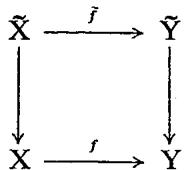
\includegraphics[keepaspectratio]{images/part001_3e847d2c.jpg}}

and compatible with the action of the group \(\{\pm1\}\) .

If \(\tilde{f}\) is an orientation of f and if \(\eta\) is an orientation of Y, there exists one and only one orientation \(\xi\) of X such that the diagram

\pandocbounded{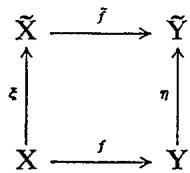
\includegraphics[keepaspectratio]{images/part001_a1f56317.jpg}}

is commutative. We say that \(\xi\) is associated with \(\eta\) by \(f\) .

Examples

\begin{enumerate}
\def\labelenumi{\alph{enumi})}
\item
  If Y is reduced to a point, an orientation of f is equivalent to an orientation of X.
\item
  Suppose \(f\) is étale. For every \(x \in X\), the map \(\mathrm{T}_{x}(f)\) is an isomorphism of \(\mathrm{T}_{x}(\mathrm{X})\) onto \(\mathrm{T}_{f(x)}(\mathrm{Y})\), and defines (by transport of structure) a bijection
\end{enumerate}

\[
\tilde {f} _ {x}: \mathrm{Or} (\mathrm{T} _ {x} (\mathrm{X})) \rightarrow \mathrm{Or} (\mathrm{T} _ {f (x)} (\mathrm{Y})).
\]

The family of \(\tilde{f}_{x}\) defines an orientation \(\tilde{f}\colon\tilde{\mathbf{X}}\to\tilde{\mathbf{Y}}\) of \(f\) , said to be canonical.

\begin{enumerate}
\def\labelenumi{\alph{enumi})}
\setcounter{enumi}{2}
\tightlist
\item
  More generally, suppose that \(f\) is a submersion, and let \(\alpha\) be an orientation of the bundle T(X/Y) (8.1.3). Let \(x\in X\) and \(\xi\) be an orientation of \(\mathrm{T}_{x}(\mathrm{X}/\mathrm{Y})\). Set \(y=f(x)\); we have an exact sequence (8.1.3)
\end{enumerate}

\[
0 \rightarrow \mathrm{T} _ {x} (\mathrm{X} / \mathrm{Y}) \rightarrow \mathrm{T} _ {x} (\mathrm{X}) \xrightarrow {\mathrm{T} _ {x} (f)} \mathrm{T} _ {y} (\mathrm{Y}) \rightarrow 0
\]

and there therefore exists one and only one orientation \(\tilde{f}_{\alpha}(\xi)\) of \(\mathrm{T}_{y}(\mathrm{Y})\) such that \(\xi = \tilde{f}_{\alpha}(\xi)\alpha(x)\) (10.2.1). The map \(\tilde{f}_{\alpha}\colon \tilde{\mathrm{X}}\to \tilde{\mathrm{Y}}\) is an orientation of \(f\), said to be associated with \(\alpha\). The map \(\alpha \mapsto \tilde{f}_{\alpha}\) is a bijection from the set of orientations of \(\mathrm{T}(\mathrm{X}/\mathrm{Y})\) onto the set of orientations of \(f\).

\begin{enumerate}
\def\labelenumi{\alph{enumi})}
\setcounter{enumi}{3}
\tightlist
\item
  If \(f: X \to Y\) is an immersion, the orientations of \(f\) correspond to the orientations of the normal bundle to \(f\) .
\end{enumerate}

10.2.6 ("Orientation of a product"). Let \(\mathbf{X}_1\) (resp. \(\mathbf{X}_2\)) be a manifold locally of finite dimension and \(\xi_1\) (resp. \(\xi_2\)) an orientation of \(\mathbf{X}_1\) (resp. \(\mathbf{X}_2\)). Let \(\mathbf{X} = \mathbf{X}_1 \times \mathbf{X}_2\). The map \((x_1, x_2) \mapsto \xi_1(x_1)\xi_2(x_2)\) (10.2.1) is an orientation of \(\mathbf{X}_1 \times \mathbf{X}_2\), called the product of the orientations \(\xi_1\) and \(\xi_2\), and denoted \(\xi_1\xi_2\), or \(\xi_1 \otimes \xi_2\).

Suppose that \(X_{i}\) (i = 1, 2) are pure of dimension \(n_{i}\). The canonical isomorphism \(X_{1} \times X_{2} \to X_{2} \times X_{1}\) transforms \(\xi_{1} \otimes \xi_{2}\) into \(\xi_{2} \otimes \xi_{1}\) (resp. into \(-\xi_{2} \otimes \xi_{1}\)) if one of the \(n_{i}\) is even (resp. if \(n_{1}\) and \(n_{2}\) are odd).

10.2.7 (“Complex case”). Let F be a finite-dimensional complex vector space and let \(F_{R}\) be the underlying real vector space. Let \(\{e_{1},\ldots,e_{m}\}\) be a basis of F; then \(\{e_{1},ie_{1},e_{2},ie_{2},\ldots,e_{m},ie_{m}\}\) is a basis of \(F_{R}\) and the orientation of \(F_{R}\) defined by the 2m-vector

\[
e _ {1} \wedge i e _ {1} \wedge e _ {2} \wedge i e _ {2} \wedge \dots \wedge e _ {m} \wedge i e _ {m}
\]

is independent of the choice of the basis \(\{e_{1},\ldots,e_{m}\}\) of F; this is called the orientation of \(F_{R}\) defined by the given complex structure. If F is the direct sum of two subspaces G and H, the orientation of \(F_{R}=G_{R}\oplus H_{R}\) is the product of the orientations of \(G_{R}\) and \(H_{R}\) .

Let X be a real manifold locally of finite dimension, equipped with an almost complex structure (8.8.3). For every \(x \in X\) let \(\xi(x)\) be the orientation of \(\mathrm{T}_{x}(\mathrm{X})\) defined by its complex structure. The map \(x \mapsto \xi(x)\) is an orientation of X, called the orientation defined by the almost complex structure. In particular, we shall equip the real analytic manifold X underlying a complex analytic manifold \(X^{c}\) , locally of finite dimension, with the orientation defined by the associated almost complex structure (8.8.6). If one replaces the given complex analytic manifold structure on X by its conjugate (5.4.12.b)), this orientation is multiplied by the function \(x \mapsto (-1)^{\dim_{x} X^{c}}\) .

10.2.8. Examples

\begin{enumerate}
\def\labelenumi{\alph{enumi})}
\tightlist
\item
  Let E be a finite-dimensional real vector space. The real analytic manifold defined by E (5.2.2) is orientable. More precisely, the map \(\xi \mapsto \xi(0)\) is a bijection from the set of orientations of this manifold onto Or(E).
\end{enumerate}

In particular, the manifold \(R^{n}\) has a canonical orientation \(\xi^{n}\) defined by the half-line \(R_{+}e_{1}\wedge\cdots\wedge e_{n}\) of \(\mathrm{Or}(\mathbf{R}^{n})\).

\begin{enumerate}
\def\labelenumi{\alph{enumi})}
\setcounter{enumi}{1}
\item
  Let X be a sphere with center 0 and radius \(\rho\) in \(\mathbf{R}^n\); it is a submanifold of \(\mathbf{R}^n\). For every \(x \in \mathbf{X}\), the space \(\mathbf{T}_x(\mathbf{R}^n) = \mathbf{R}^n\) is the direct sum of the line \(\mathbf{R}x\) and of the hyperplane \(\mathbf{T}_x(\mathbf{X})\). Let \(\eta_x\) be the orientation \(\mathbf{R}_+x\) of \(\mathbf{R}x\) (“outward normal”) and let \(\xi_x\) be the unique orientation of \(\mathbf{T}_x(\mathbf{X})\) such that the product of \(\eta_x\) and \(\xi_x\) is the orientation \(\xi^n\) of \(\mathbf{R}^n\). The map \(x \mapsto \xi_x\) is an orientation of \(\mathbf{X}\), said to be canonical.
\item
  Let X be a connected manifold, and let G be a discrete group acting properly and freely on X. For X/G to be orientable, it is necessary and sufficient that X be orientable and that the action of G on the set of orientations of X be trivial.
\item
  Real projective space \(\mathbf{P}_{n-1}(\mathbf{R})\) is identified with the quotient of the sphere \(S_{n-1}\) by the group \(\{\pm1\}\) acting by \(x\mapsto\pm x\) ; it is orientable if n is even, and non-orientable if n is odd.
\item
  Every quotient of a Lie group by a connected Lie subgroup is orientable.
\end{enumerate}

